\chapter{Конструкторский раздел}
\label{cha:design}

\section{Архитектура программного продукта}

Разрабатываемый метод состоит из 2 частей:

\begin{enumerate}
	\item модуль предобработки входных данных;
	\item модуль классификации жестового символа.
\end{enumerate}

В качестве входных данных используются RGB изображения. Данный формат данных может быть получен с любого фото- и видео-устройства.

\section{Предобработка изображений}

В рассмотренном ранее методе выделения силуэта кисти руки предлагалась фильтрация пикселей изображения в цветовом пространстве YCbCr. Как показывает практика, данное решение имеет недостаток в виде артефактов выделения. Данная проблема возникает из-за наличия в фоновой части изображения пикселей, цвет которых близок к цвету кожи в данном цветовом пространстве.

Избежать подобные дефекты можно через дополнительную фильтрацию в цветовом пространстве HSV\cite{Kolkur}. В итоговом методе пиксели исходного изображения проверяются одновременно и в обоих цветовых пространствах. 

Для преобразования изображения из RGB в YCbCr используется формула \ref{eq:ycbcr}.

\begin{eqnarray}\label{eq:ycbcr}
\begin{bmatrix}
Y\\Cb\\Cr
\end{bmatrix}
=
\begin{bmatrix}
16\\128\\128
\end{bmatrix}
+
\begin{bmatrix}
65,81 & 128,551 & 24,966 \\
-37,797 & -74,203 & 112\\
112 & -93,786 & -18,214
\end{bmatrix}
\begin{bmatrix}
R\\G\\B
\end{bmatrix}
\end{eqnarray}

В HSV координатами цвета являются:

\begin{itemize}
	\item H -- цветовой тон, интервал значений $0 - 360^\circ$;
	\item S -- насыщенность, $0 - 1$;
	\item V -- яркость, $0 - 1$;
\end{itemize}

Для получение значения координат пикселя в пространстве HSV, нормализуем его координаты в RGB по максимальному значению.
\begin{equation}
R'=R/255 \quad G'=G/255 \quad B'=B/255
\end{equation}

Зададим так же 
\begin{equation}
C_{max} = max(R', G', B')
\end{equation}

\begin{equation}
C_{min} = min(R', G', B')
\end{equation}

\begin{equation}
\Delta = C_{max} - C_{min}.
\end{equation}

Тогда координаты пикселя в пространстве HSV вычисляются следующим образом:

\begin{eqnarray}
\begin{matrix}
H & =
& \left\{
\begin{matrix}
0^\circ &, \Delta = 0 \\
60^\circ \times ( \frac{G' - B'}{\Delta} \mod 6 )& , C_{max} = R' \\
60^\circ \times ( \frac{B' - R'}{\Delta} + 2)& , C_{max} = G' \\
60^\circ \times ( \frac{R' - G'}{\Delta} + 4)& , C_{max} = B' \\
\end{matrix} \right.
\end{matrix}
\end{eqnarray}

\begin{eqnarray}
\begin{matrix}
S & =
& \left\{
\begin{matrix}
0 &, C_{max} = 0 \\
\frac{\Delta}{C_{max}} &,C_{max} \ne 0
\end{matrix} \right.
\end{matrix}
\end{eqnarray}

\begin{eqnarray}
V = C_{max}
\end{eqnarray}

Алгоритм \ref{des:image_mask} описывает процесс получения силуэта кисти руки.

\begin{algorithm}[H]
	\label{des:image_mask}
	\SetAlgoLined
	\KwIn{Изображение $x$}
	\KwOut{Однотонное черно-белое изображение $y$}	
	
	Получить изображение в YCbCr
	
	$x_{ycbcr} \leftarrow YCbCr(x)$
	
	Получить изображение в HSV
	
	$x_{hsv} \leftarrow HSV(x)$
	
	\ForEach{пикселя p изображения x с координатами i, j}{
		$Y =$ значение $Y$ пикселя $x_{ycbcr}$
		
		$Cb =$ значение  $Cb$ пикселя $x_{ycbcr}$
		
		$Cr =$ значение  $Cr$ пикселя $x_{ycbcr}$
		
		$H =$ значение $H$ пикселя $x_{hsv}$
		
		$S =$ значение  $S$ пикселя $x_{hsv}$
		
		$V =$ значение  $V$ пикселя $x_{hsv}$
		
		\If{
			$Y > 80$ и
			$ 135 \le Cr \le 180 $ и
			$ 85 \le Cb \le 135 $ и
			$ H \le 50^\circ $ и 
			$ 0,23 \le S \le 0,68 $
		}{
			$y[i][j] = 255$
		} \Else{
			$y[i][j] = 0$
		}
	}
	
	\caption{Алгоритм выделения силуэта кисти руки}
\end{algorithm}

\section{Классификация жестовых символов}

Ранее было показано преимущество использование СНС в качестве классификатора в известных методах распознавания жестовых символов, выделены недостатки данного метода. Предложено использование КНС в качестве альтернативы с целью уменьшения обучающей выборки, ускорения процесса обучения и добавления методу инвариантности к аффинным преобразованиям изображения.

\subsection{Алгоритм передачи данных между капсульными слоями}

Передача информации между капсульными слоями происходит с помощью динамической маршрутизации. Целью данного алгоритма является передача выхода низкоуровневых капсул только тем капсулам, которые способны на основании полученных данных получить наилучший результат в контексте решаемой данной архитектурой задачи. 

Все входные вектора капсулы после аффинного преобразования умножаются на коэффициенты маршрутизации, сумма которых равна единице. Значения данных коэффициентов задаются функцией softmax (формула \ref{eq:softmax}).

\begin{equation}\label{eq:softmax}
c_{ij} = \frac{e^{b_{ij}}}{\sum_{k}e^{b_{ik}}}
\end{equation}

Значение неизвестных $b_{ij}$ вычисляются дискриминативно одновременно с остальными весовыми коэффициентами. Данный процесс зависит исключительно от взаимного расположения и типа капсул и не зависит от входных данных. Начальные коэффициенты связи затем итеративно уточняются на основании согласованности текущих выходов $v_j$ низкоуровневых капсул $j$ и предсказанием $\hat{u}_{i|j}$ высокоуровневой капсулы $i$.

Согласованность между капсулами определяется скалярным произведением $a_{ij} = v_j \hat{u}_{j|i}$. Оно рассматривается как логарифмическая вероятность и добавляется к исходному значению $b_{ij}$  перед вычислением новых значений для всех коэффициентов связи, связывающих капсулу $i$ с капсулами более низкого уровня.

Алгоритм \ref{alg:routing} описывает итерационный процесс вычисления коэффициентов связи.

\begin{algorithm}[H]
	\label{alg:routing}
	\SetAlgoLined
	\KwIn{Вектор $\hat{u}_{j|i}$, количество итераций $r$, капсульный слой $l$}
	\ForEach{индекса $i$ капсулы слоя $l$ и индекса $j$ капсулы слоя $l+1$}{$b_{ij} \leftarrow 0$}
	\For{ r итераций}{
		\ForEach{индекса $i$ капсулы слоя $l$}{$c_{ij} \leftarrow softmax(b_{ij})$}
		\ForEach{индекса $j$ капсулы слоя $l+1$}{$s_j = \sum_{i}c_{ij}\hat{u}_{j|i}$}
		\ForEach{индекса $j$ капсулы слоя $l+1$}{$v_j=\frac{{||s_j||}^2}{1 + {||s_j||}^2}\frac{s_j}{||s_j||}$}
		\ForEach{индекса $i$ капсулы слоя $l$ и индекса $j$ капсулы слоя $l+1$}{$b_{ij} \leftarrow b_{ij} + v_j \hat{u}_{j|i}$}
	}
	\caption{Алгоритм динамической маршрутизации}
\end{algorithm}


\subsection{Архитектура сети}

Архитектура сети состоит из 4 слоев:

\begin{enumerate}
	\item Входной слой. На вход сети подается черно-белое одноканальное изображение, где каждое значение пикселя означает интенсивность белого цвета.
	\item Сверточный слой. Имеет 256 фильтров размерностью $9 \times 9$ со смещением 1.	В качестве активационной функции используется ReLU (формула \ref{anal:relu}).
	\begin{equation}
	x_{k} = \max(u_{k}, 0), k = 1, ..., K
	\label{anal:relu}
	\end{equation}
	где 
	\begin{itemize}
		\item $x_k$ -- выходное значение нейрона $k$-го слоя;
		\item $u_k$ -- результат работы сумматора нейрона $k$-го слоя.
	\end{itemize}
	\item Первый капсульный слой. Состоит из 32 капсул, каждая из которых представляет собой набор из 8 сверточных слоев с дает на выходе $N \times N$ векторов длины 8, где $N$ - число строк или столбцов матрицы, полученной в результате свертки. Ядро свертки имеет размерность $9 \times 9$ со смещением 2. Условно, данную капсулу можно представить в виде группы подкапсул, объединенных одним набором весовых коэффициентов.
	\item Выходной капсульный слой. Состоит из $J$ капсул, где $J$ -- количество классов. Выходной вектор имеет длину 8. Каждая капсула принимает на вход все выходы с предыдущего слоя с применением алгоритма динамической маршрутизации. Для большей наглядности данный слой можно интерпретировать как полносвязный в СНС. Длина выходного вектора капсулы на данном слое соответствует вероятности принадлежности входных данных к классу, представленному конкретной капсулой, то есть итоговый класс изображения определяется по капсуле с выходным вектором наибольшей длины.
\end{enumerate}

Схема нейронной сети представлена на рисунке \ref{design:CapsNet}.

\begin{figure}
	\centering
	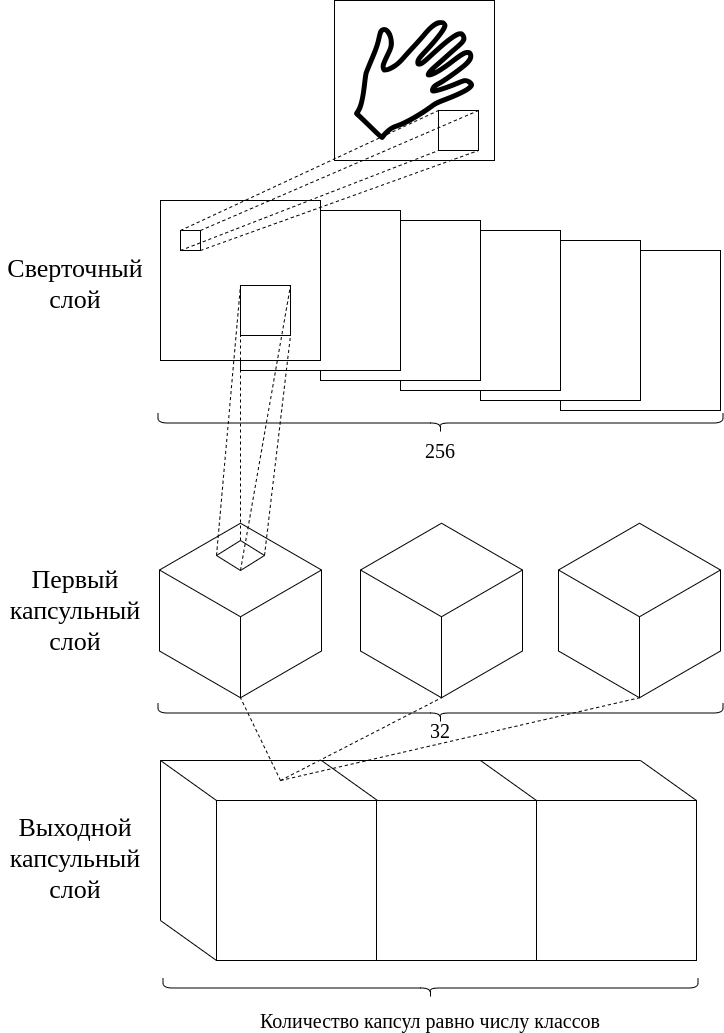
\includegraphics[width=\textwidth]{inc/img/CapsNet}
	\caption{Архитектура капсульной нейронной сети}
	\label{design:CapsNet}
\end{figure}

Ошибка обучения вычисляется для каждой капсулы выходного слоя по следующей формуле:

\begin{equation}
\label{eq:magin-loss}
L_k = T_k \max (0, m^+ - ||v_k||)^2 + \lambda (1 - T_k) \max (0, ||v_k|| - m^-)^2
\end{equation}

где

\begin{itemize}
	\item $L_k$ -- ошибка $k$ - ой капсулы;
	\item $T_k$ равен 1, если $k$-я капсула представляет текущий класс, иначе равен 0;
	\item $m^+, m^-$ -- варьируемые коэффициенты. В данной работе использовались значения 0,9 и 0,1 соответственно;
	\item $\lambda$ -- коэффициент уменьшения исходных весов для отсутствующих классов, исключающий из процесса обучения сокращение длины вектора активности для всех сущностей. В данной работе используется значение 0,5.
\end{itemize}

Итоговая ошибка обучения вычисляется как сумма $L = \sum_{k} L_k$.

\section{Вывод}

В конструкторском разделе описывается построение метода распознавания жестовых символов. Дано подробное описание, построены схемы выбранных алгоритмов. При этом выделены основные этапы работы метода с указанием необходимых исходных данных для его работы и полученных результатов на каждом этапе.